\chapter{Outline and Contributions}

\begin{figure}[H]
    \centering
    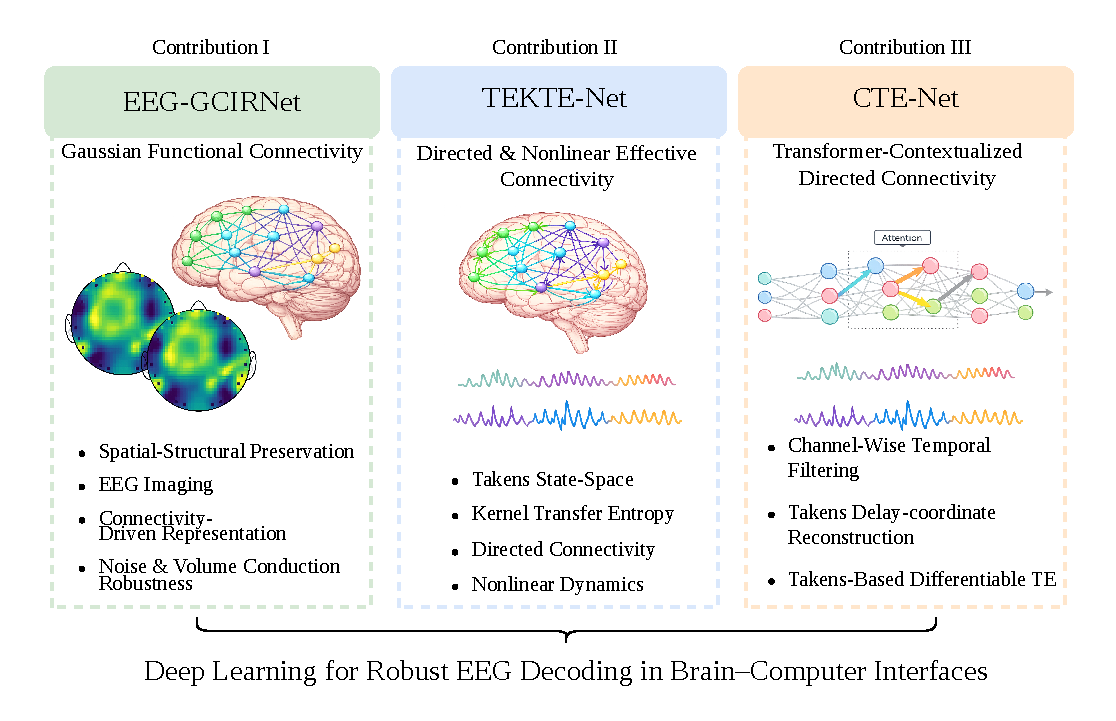
\includegraphics[width=\linewidth]{Figures/contributions.pdf}
    \caption{The three methodological contributions address robustness, interpretability, and generalization in \gls{eeg}-based \gls{bci} systems through connectivity-driven representations, nonlinear and directed predictive-dependency modeling, and Transformer-based contextualization.}
    \label{fig:contributions}
\end{figure}

This chapter presents a concise overview of the three methodological contributions developed in this doctoral thesis. The work is structured around methodological frameworks aimed at strengthening the robustness, interpretability, and generalization of \gls{eeg}-based \gls{bci} systems, considering the inherently noisy and highly variable nature of \gls{eeg} signals. The three contributions are grounded in peer-reviewed journal articles published by the author and are incorporated into a unified doctoral research framework in accordance with the intellectual property regulations of the Universidad Nacional de Colombia, available in the \href{https://unal.edu.co/archivos/user_upload/docs/legal.pdf}{Acuerdo 035 de 2003 del Consejo Académico}, and with the copyright and licensing policies of the respective publishers, including MDPI and Elsevier. An overview of the three contributions and their relationship with robustness, interpretability, and generalization is presented in Figure~\ref{fig:contributions}.

The first contribution, entitled \textbf{Gaussian Connectivity-Driven \gls{eeg} Imaging for Deep Learning-Based \gls{mi} Classification}, is based on the peer-reviewed article ``A Gaussian Connectivity-Driven EEG Imaging for Deep Learning-Based Motor Imagery Classification'' (Sensors, 2026). This contribution proposes a Gaussian connectivity-driven representation for constructing \gls{eeg} images that preserve spatial and structural relationships between channels. The proposed framework enables the integration of functional connectivity information within deep learning architectures, addressing limitations of traditional approaches based on local or channel-independent features and promoting improved discrimination of relevant neurophysiological patterns under conditions of noise, source mixing, and low spatial resolution.

The second contribution, entitled \textbf{Takens-Based Kernel \gls{te} Connectivity Network for \gls{mi} Classification}, is based on the peer-reviewed article ``Takens-Based Kernel Transfer Entropy Connectivity Network for Motor Imagery Classification'' (Sensors, 2025). This contribution extends the previous line of research by explicitly addressing nonlinear, directed, and time-dependent dependencies between \gls{eeg} signals. Through state-space reconstruction and kernel-based \gls{te} estimation, the proposed framework provides a richer characterization of directed predictive dependencies and dynamic information exchange between \gls{eeg} channels, capturing interactions that cannot be adequately represented by symmetric or static connectivity measures.

The third contribution, entitled \textbf{Transformer-Based Modeling of Directed Transfer Entropy Connectivity for EEG-Based ADHD Classification in Children}, is based on the peer-reviewed article ``Transformer-Based Modeling of Directed Transfer Entropy Connectivity for EEG-Based ADHD Classification in Children'' (Sensors, 2026). This contribution introduces CTE-Net, an end-to-end architecture that integrates Transformer-based contextualization, channel-wise nonlinear temporal filtering, Takens delay-coordinate reconstruction, and differentiable kernel-based \gls{te} estimation. The framework was developed to learn directed-connectivity representations from pediatric \gls{eeg} and was evaluated for the classification of children with \gls{adhd} and controls using subject-wise partitions and repeated training. In addition to predictive performance, this contribution examines the effects of the Transformer and \gls{te} components through ablation experiments and evaluates the organization, within-participant dispersion, and stability of the learned representations.

\subsection{Tested Datasets}\label{sec:datasets2}

To evaluate the effectiveness and robustness of the proposed methodology, extensive experiments were conducted using four \gls{eeg} datasets that are widely adopted in \gls{bci} research. Specifically, two binary \gls{mi} classification scenarios were considered using the \textit{GIGA MI} dataset and the \textit{BCI Competition IV 2a} dataset in their bi-class configurations. Additionally, the \textit{PhysioNet \gls{eeg} Motor Movement/Imagery} dataset was employed to address a multi-class \gls{mi} classification problem, allowing the assessment of the proposed approach under increased task complexity. Finally, the generalization capability of the methodology was evaluated on the \textit{\gls{eeg} data for \gls{adhd}/control children} dataset, which represents a clinical classification scenario aimed at distinguishing between children with \gls{adhd} and healthy control subjects.

\begin{itemize}
    \item[--] \textit{GIGAScience Dataset for \gls{eeg}-based \gls{mi}:} The GIGAScience \gls{mi} dataset, publicly available at \url{http://gigadb.org/dataset/100295} (accessed on 1 July 2025), provides one of the most comprehensive \gls{eeg} corpora for \gls{mi} analysis. The dataset comprises recordings from 52 healthy participants (50 with usable data), each performing a single \gls{eeg}-\gls{mi} session. Every session consists of five to six experimental blocks, with each block containing approximately 100–120 trials per class. Each trial spans seven seconds and follows a fixed timeline: an initial blank screen (0–2~s), a visual cue indicating either left- or right-hand \gls{mi} (2–5~s), and a concluding blank interval (5–7~s). Inter-trial intervals vary randomly between 0.1~s and 0.8~s to mitigate anticipatory bias, as illustrated in Figure~\ref{fig:giga_timeline}.

    \begin{figure}[htbp]
      \centering
      \input{Figures/GigaScience}
      \caption{Experimental timeline of the GigaScience \gls{mi}-\gls{eeg} dataset.}
      \label{fig:giga_timeline}
    \end{figure}    
    
    \gls{eeg} signals were recorded at a sampling frequency of 512~Hz using a 64-channel cap arranged according to the international 10--10 electrode placement system see Figure~\ref{fig:giga_montage}. In addition to the \gls{mi} sessions, the dataset includes recordings of real motor execution and six auxiliary non-task-related events—eye blinks, vertical and horizontal eye movements, head motions, jaw clenching, and resting state—enabling a broader exploration of \gls{eeg} noise sources and artifact correction. This multimodal composition makes the GigaScience particularly valuable for benchmarking advanced deep learning and connectivity-based \gls{eeg} decoding frameworks, as it supports both intra-subject and inter-subject generalization studies.

    \begin{figure}[htbp]
      \centering
      \resizebox{0.4\linewidth}{!}{\input{Figures/Giga}}
      \caption{Electrode montage, where colors indicate scalp regions:
      \protect\legend{frontal_left} Frontal left;
      \protect\legend{frontal} Frontal;
      \protect\legend{frontal_right} Frontal right;
      \protect\legend{central_left} Central left;
      \protect\legend{central_right} Central right;
      \protect\legend{posterior_left} Posterior left;
      \protect\legend{posterior} Posterior;
      \protect\legend{posterior_right} Posterior right.} 
      \label{fig:giga_montage}
    \end{figure}

    \item[--] \textit{\gls{bci} Competition IV dataset 2a:} a publicly available resource composed of \gls{eeg} recordings from nine healthy participants. These recordings were obtained during multiple trials of a (\gls{mi}) experiment with the protocol illustrated in~\Cref{fig:bci2a}. In each trial, participants first see a fixation cross on a computer screen, accompanied by an auditory cue. Two seconds later, a directional arrow appears for 1.25 seconds, signaling the start ($t=0$) of one of four possible \gls{mi} tasks: left-hand, right-hand, both feet, or tongue movement. One second after the \gls{mi} signal, subjects begin performing the instructed task during three seconds (i.e., until the 4-seconds mark after the instruction), at which point the cross disappears. A brief 1.5-second pause follows, during which the screen remains blank. For validation purposes, this study excludes feet and tongue movement tasks and focuses solely on binary classification of trials instructed to move the left ($y=0$) and right ($y=1$) hands. For each subject, the \gls{bci} Competition IV provides two subsets with the same experimental protocol: the training subset holds between 113 and 138 trials per subject, and the testing subset holds between 108 and 142 per subject~\cite{tangermann2012review}.
    
    \begin{figure}[htbp]
      \centering
      % Carga y escala al 90% del ancho de texto
      \resizebox{0.9\textwidth}{!}{\input{Figures/BCI2a.tex}}
      \caption{Schematic description of the \gls{mi} paradigms.}
      \label{fig:bci2a}
    \end{figure}

    The \gls{eeg} data were recorded using $C=22$ Ag/AgCl electrodes, placed according to the international 10/20 system as shown in~\Cref{fig:topoplot}. The data preprocessing applies a 50~Hz notch filter and a bandpass filter between 0.5 and 100~Hz and resamples to 250~Hz. Therefore, each participant comprises a subset of 22 channels and $N$ samples, and classification is based solely on labels 1 and 2, which distinguish between right-hand and left-hand \gls{mi}, respectively. Trials are split into two-seconds windows with 0.5 seconds overlap, that is $T=500$, from which the segments from 2.0 to 4.0 seconds after cue onset are selected to train the model as they are expected to hold the most relevant information to the \gls{mi} task. Lastly, the spherical splines method applies the surface Laplacian transform to each segment to reduce the influence of low spatial frequency activity, minimize the occurrence of spurious channel connectivities, and mitigate the volume conduction effect~\cite{tenke2015surface, hua2024scalp,lu2012adaptive, kapralov2024sensorimotor}.

    \begin{figure}[htbp]
      \centering
      
      \resizebox{0.5\textwidth}{!}{\input{Figures/electrodes}}
      \caption{Sensor positions according the 10--20 electrode placement system for the \gls{bci} Competition IV 2a dataset. 22 channels are distributed over ten main brain regions: \legend{frontal_left} Frontal left,\legend{frontal} Frontal,\legend{frontal_right} Frontal right,\legend{central_left} Central left,\legend{central_right} Central right,\legend{centro_parietal_left} Centro-parietal left,\legend{centro_parietal_right} Centro-parietal right,\legend{parietal_left} Parietal left,\legend{parietal_right} Parietal right,\legend{posterior} Posterior.}\label{fig:topoplot}
    \end{figure}
    
    \item[--] \textit{\gls{eeg} Motor Movement/Imagery Database:}The \gls{eegmmidb} \cite{physionet}, available at \url{https://physionet.org/content/eegmmidb/1.0.0/} (accessed on 7 December 2025), was employed as a secondary benchmark to evaluate the framework's versatility. This dataset comprises electroencephalographic recordings from 109 healthy participants performing a variety of real and imagined motor tasks. The \gls{eeg} signals were acquired using 64 scalp electrodes positioned according to the international 10--10 system see Figure~\ref{fig:giga_montage} and sampled at 160~Hz. The recording protocol encompasses 14 sessions per subject, including resting-state conditions, motor execution tasks, and \gls{mi} tasks. Data segmentation was performed based on event annotations to define discrete trials. Each trial corresponds to a 4.1~s window, yielding a raw input matrix of $64 \text{ channels} \times 640 \text{ samples}$. 
    
    To standardize the classification
    task, the original PhysioNet labels (0--11) were reorganized into five classes following a physiological interpretation of \gls{mi} tasks: (1) Left Hand \gls{mi} (labels 0 and 2); (2) Right Hand \gls{mi} (labels 1 and 3); (3) Both Fists \gls{mi} (labels 4 and 6); (4) Both Feet \gls{mi} (labels 5 and 7); and (5) Rest (label 11). Motor execution trials (label 10) and tongue \gls{mi} events (labels 8 and 9) were excluded from the analysis. In alignment with the experimental design of the GigaScience dataset, only \gls{mi}-related sessions and resting-state segments were considered. The experimental configuration is summarized in Figure~\ref{fig:physionet}.

    \begin{figure}[htbp]
     \centering
      % Paleta pastel alternativa
\definecolor{FixationColor}{HTML}{BFD8B8}
\definecolor{MotorColor}{HTML}{F6C28B}
\definecolor{RestColor}{HTML}{A7C5EB}
\definecolor{InterColor}{HTML}{EDE6F2}
\definecolor{CueColor}{HTML}{B5EAEA}

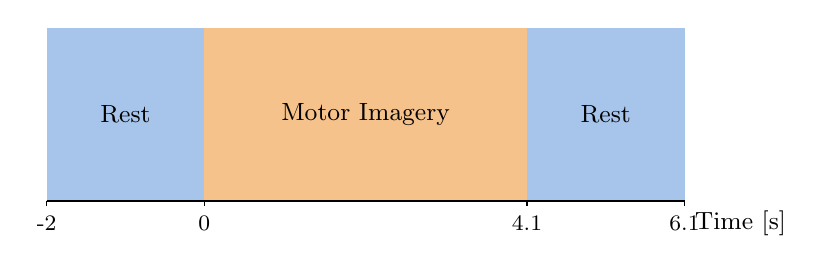
\begin{tikzpicture}
  % ===== Parámetros =====
  \def\boxheight{2.2}

  % Tiempos (s)
  \def\startRest{-2}
  \def\endRestA{0}
  \def\endMI{4.1}
  \def\endRestB{6.1}

  % ===== Bloques (SIN MARCOS) =====
  \fill[RestColor]  (\startRest,0) rectangle (\endRestA,\boxheight);
  \fill[MotorColor] (\endRestA,0)  rectangle (\endMI,\boxheight);
  \fill[RestColor]  (\endMI,0)     rectangle (\endRestB,\boxheight);

  % ===== Etiquetas internas =====
  \node[font=\small] at ({(\startRest+\endRestA)/2},{0.5*\boxheight}) {Rest};
  \node[font=\small] at ({(\endRestA+\endMI)/2},{0.5*\boxheight}) {Motor Imagery};
  \node[font=\small] at ({(\endMI+\endRestB)/2},{0.5*\boxheight}) {Rest};

  % ===== Eje X =====
  \draw[thick] (\startRest,0) -- (\endRestB,0)
        node[below right,font=\small] {Time [s]};

  \foreach \x/\lbl in {
      \startRest/-2,
      \endRestA/0,
      \endMI/4.1,
      \endRestB/6.1}{
    \draw (\x,0) -- ++(0,-2pt) node[below,font=\footnotesize] {\lbl};
  }

\end{tikzpicture}

      \caption{Overview of the \gls{eegmmidb} \gls{mi}-\gls{eeg} dataset: experimental timeline.}
      \label{fig:physionet}
    \end{figure}

    \item[--] \textit{\gls{adhd}/control children:}
    In this study, we use the publicly available \textit{\gls{eeg} data for \gls{adhd}/control children} dataset, collected and shared by Nasrabadi \textit{et al.} via IEEE DataPort~\cite{nasrabadi2020eeg}. The database comprises \gls{eeg} recordings from 121 school-aged children between 7 and 12 years old, including 61 diagnosed with \gls{adhd} and 60 typically developing control subjects~\cite{ekhlasi2021pte,li2025gcn}. \gls{adhd} diagnoses were established by an experienced child psychiatrist according to \gls{dsmiv} criteria. At the time of recording, patients had been treated with methylphenidate (Ritalin) for up to six months, whereas children in the control group had no history of psychiatric or neurological disorders, including epilepsy, or high-risk behaviors~\cite{ekhlasi2021pte,li2025gcn}.

    \begin{figure}[H]
      \centering
      \resizebox{0.5\textwidth}{!}{\input{Figures/TDHA Montage}}
     \caption{Scalp electrode montage following the international 10--20 system for the \gls{adhd}/control children dataset. The 19 \gls{eeg} channels are grouped into anatomically defined cortical regions, indicated by color: \legend{PurpleLeftSide} frontal left and central left, \legend{ElecBG} midline electrodes (Fz, Cz, Pz), \legend{Purple} frontal right, \legend{BlueRightSide} central right, \legend{GreenC} centro-parietal and parietal left, \legend{Orange} centro-parietal and parietal right, and \legend{UpperGreen} occipital region.}
    \label{fig:TDHA}
    \end{figure}
    
    \gls{eeg} signals were recorded while participants performed a visually guided attention task designed to probe attentional deficits associated with \gls{adhd}~\cite{ekhlasi2021pte,diagnosticInterface2024}. During the task, children were presented with a sequence of cartoon images containing a variable number of characters (ranging from 5 to 16 per image; see \Cref{fig:example}) and were instructed to silently count the number of Figures in each scene. Stimuli were displayed continuously, with each new image appearing immediately after the participant’s response, resulting in variable recording lengths depending on individual response times~\cite{li2025gcn,diagnosticInterface2024}.

    \begin{figure}[htbp]
    \centering
    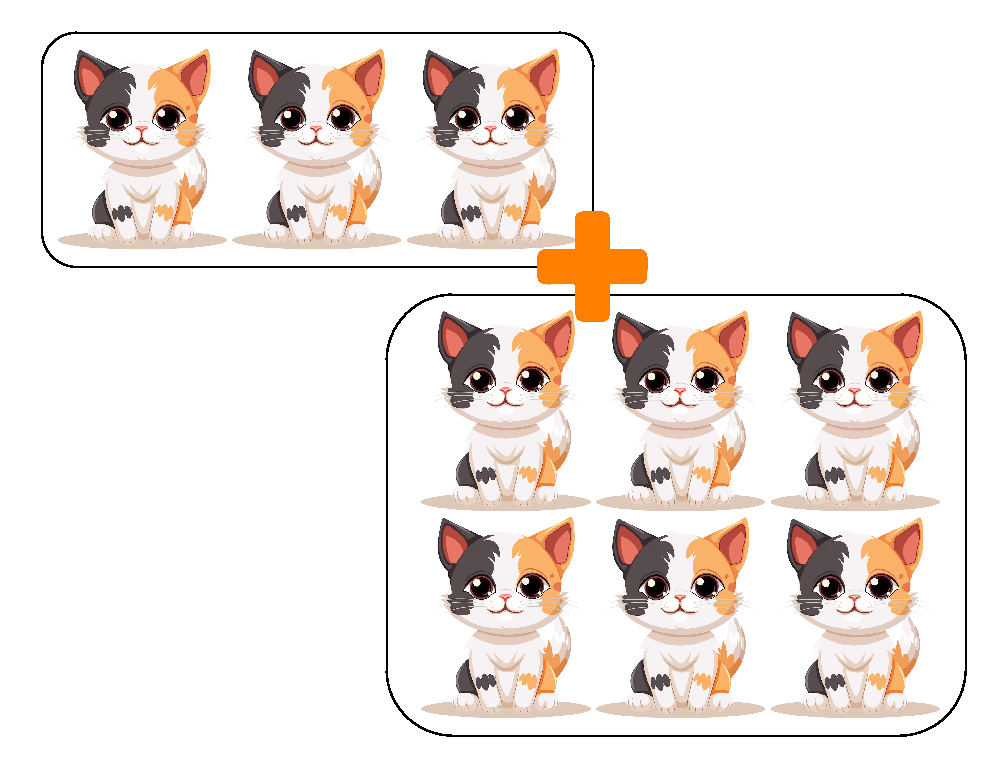
\includegraphics[width=0.7\linewidth]{Figures/TDHA.pdf}
    \caption{Example of the visual stimuli shown to
    children during \gls{eeg} recording.}
    \label{fig:example}
    \end{figure}

    \gls{eeg} recordings were acquired using 19 scalp electrodes placed according to the international 10--20 system (Fp1, Fp2, F3, F4, F7, F8, Fz, C3, C4, Cz, P3, P4, Pz, T3/T7, T4/T8, T5/P7, T6/P8, O1, O2; see \Cref{fig:TDHA}) at a sampling frequency of 128~Hz~\cite{nasrabadi2020eeg,diagnosticInterface2024,li2025gcn}. This dataset has been extensively used in effective connectivity studies based on Phase Transfer Entropy (\gls{pte}/\gls{dpte}) and multivariate \gls{te} to characterize altered directed information flow and short- and long-range connectivity patterns in \gls{adhd}~\cite{ekhlasi2021pte,ekhlasi2025omute,ekhlasi2021classification}.

    Following previous connectivity-based analyses, a standardized preprocessing pipeline was implemented using \gls{eeglab}~\cite{delorme2004eeglab,li2025gcn}. \gls{eeg} signals were re-referenced and calibrated to standard electrode coordinates, band-pass filtered between 0.5 and 60~Hz, and retained at a sampling frequency of 128~Hz. Artifacts related to eye blinks, muscle activity, and line noise were identified and removed using independent component analysis (\gls{ica}) combined with automatic component labeling (e.g., \gls{iclabel})~\cite{li2025gcn,delorme2004eeglab}. The cleaned continuous recordings were subsequently segmented into non-overlapping 5-s epochs, yielding a large set of artifact-free multi-channel segments for connectivity estimation and model training~\cite{li2025gcn,ekhlasi2021pte}.

    
\end{itemize}
